\chapter{Применение разработанной нечеткой модели для прогнозирования временных рядов в задачах экономики и финансов}

Прогнозирование временных рядов в экономике и финансах играет ключевую роль как инструмент анализа и предсказания динамики последовательно изменяющихся данных. Оно служит основой для принятия обоснованных решений в условиях неопределенности, обеспечивая оценку будущих тенденций, рисков и возможностей. Это позволяет субъектам экономической и финансовой деятельности — от индивидуальных инвесторов до государственных структур — оптимизировать управление ресурсами, минимизировать потери и формировать долгосрочные стратегии.

Стратегическое планирование и бюджетирование (обоснование финансовых планов, оптимизация ресурсного распределения), Управление рисками и инвестиционные решения

В государственных и корпоративных бюджетах прогнозы временных рядов используются для оценки объёмов доходов и расходов, планирования денежных потоков и определения ключевых показателей эффективности. У компаний прогнозирование сезонных и трендовых колебаний продаж помогает корректировать производственные мощности, склады и персонал, тем самым минимизируя издержки и снижая риск дефицита или перепроизводства. Прогнозы временных рядов служат основой для разработки моделей оптимального распределения активов и стратегий ребалансировки портфеля в зависимости от ожидаемых рыночных движений.

Одномерные модели оправданы, когда целевой ряд обладает высокой автокорреляцией, слабо зависит или отсутствует информация о значениях внешних факторов, ограниченны вычислительные и временные ресурсы для оценки взаимосвязей измерений. Примеры: краткосрочное прогнозирование инфляции, прогнозирование индекса S\&P 500. Многомерные методы необходимы, когда влияние других временных рядов или внешних предикторов существенно для точности прогноза, доступна качественная информация об этих переменных или когда доступна информация о их будущих значениях, а также когда необходимо исследовать влияние <<шока>> в одной переменной на остальные. Примеры: оценка влияния нефтяных шоков на экономику Нигерии.

\todo{Область и ситуации в которой применима разработанная модель (авторегрессионная)}

\todo{Для прогнозирования используются модели}

\section{Задача прогнозирования стоимости ценных бумаг Тайванской биржи}

\cite{Sadaei2016}

Taiwan Capitalization Weighted Stock Index (TWSE) - популярный набор данных стоимости акций биржи TAIEX, исполюзуемый для оценки качества прогнозирования временных рядов. Датасет предоставляется официальным сайтом  Набор данных составлен из ежедневных значений цены индекса в момент закрытия биржи в промежутке от 2001 до 2022 года.

\begin{figure}[hbt] 	
	\label{fig:twse-ns-fuzzification}
	\centering
	%\includegraphics[width=\textwidth]{twse-ns-fuzzification}
	\caption{Тренировочный и тестовый отрезок значений временного ряда TWSE и среднеквадратичное отклонение гауссовой ф. п. в каждой точке.}
\end{figure}

 Для оценки качества были отложены последние 500 окон временных точек, а для построения базы правил использовались предшествующие им 1000 окон. Отрезки исходного временного ряда для тестовый и тренировочный выбирались таким образом, чтобы диапазон значений в тестовом отрезке был включен в диапазон тренировочного отрезка. Фаззификация временного ряда состояла в построении гауссовой функции принадлежности в каждой точке временного ряда. Центры гауссовой функции принадлежности равны значениям временного ряда в каждой точке. Значение среднеквадратичного отклонения находится согласно способу описанному в разделе \ref{} главы \ref{}: \todo{уточнить}.
 
 \begin{figure}[hbt] 	
 	\label{fig:twse-optuna-parallel-score}
 	\centering
 	%\includegraphics[width=\textwidth]{twse-optuna-parallel}
 	\caption{Влияние комбинации значений гиперпараметров на значение оптимизируемой метрики.}
 \end{figure}
 
В рамках данной задачи горизонт прогнозирования задается равным 1. В качестве функции приспособленности использовалась метрика \todo{NDEI}.

Для оценки предельных возможностей непосредственно нечеткой логической модели в данной задаче параметры $\alpha,\dots$ подбирались с помощью байесовской оптимизации, реализованной в Python-библиотеке Optuna \cite{Optuna2024, akiba2019optuna}. \todo{Диапазоны значений этих параметров, в пределах которых производился поиск оптимальной комбинации, приведены в таблице}. Для сокращения длительности байесовой оптимизации размер популяции выбирался равным количеству правил в базе правил, а число итераций ролевого алгоритма подбора базы правил --- 50. Для алгоритма Gradient-aware PSO в методе дефаззификации MeOM размер популяции составляет 30 особей, а количество итераций --- 100. График значений оптимизируемой метрики для различных комбинаций значений гиперпараметров нечеткой модели в параллельных координатах изображен на рисунке \cref{fig:twse-optuna-parallel-score}. Из него можно отметить несколько наблюдений. При значение параметра лага $p = 5$, значении коэффициента среднеквадратичного отклонения функций принадлежности для фаззифицированных входных данных $\phi = 0.1$ и количестве правил в базе правил $N = 50$ обеспечивается лучшее значение целевой метрики. Также лучшее качество прогнозирования на тренировочном отрезке временного ряда достигается при использовании нечеткой импликации \textit{Лукасевича} и метода дефаззфикации --- \textit{MeOM}.

\begin{figure}[hbt] 	
	\label{fig:twse-optuna-parallel-duration}
	\centering
	%\includegraphics[width=\textwidth]{twse-optuna-parallel}
	\caption{Влияние комбинации значений гиперпараметров на время построения базы правил.}
\end{figure}

На рисунке \cref{fig:twse-optuna-parallel-duration} график изображает зависимость времени оптимизации базы правил нечеткой системы при тех же комбинациях гиперпараметров, что и на рисунке \cref{fig:twse-optuna-parallel-score}.

\begin{figure}[hbt] 	
	\label{fig:twse-rules-pso-optimization}
	\centering
	%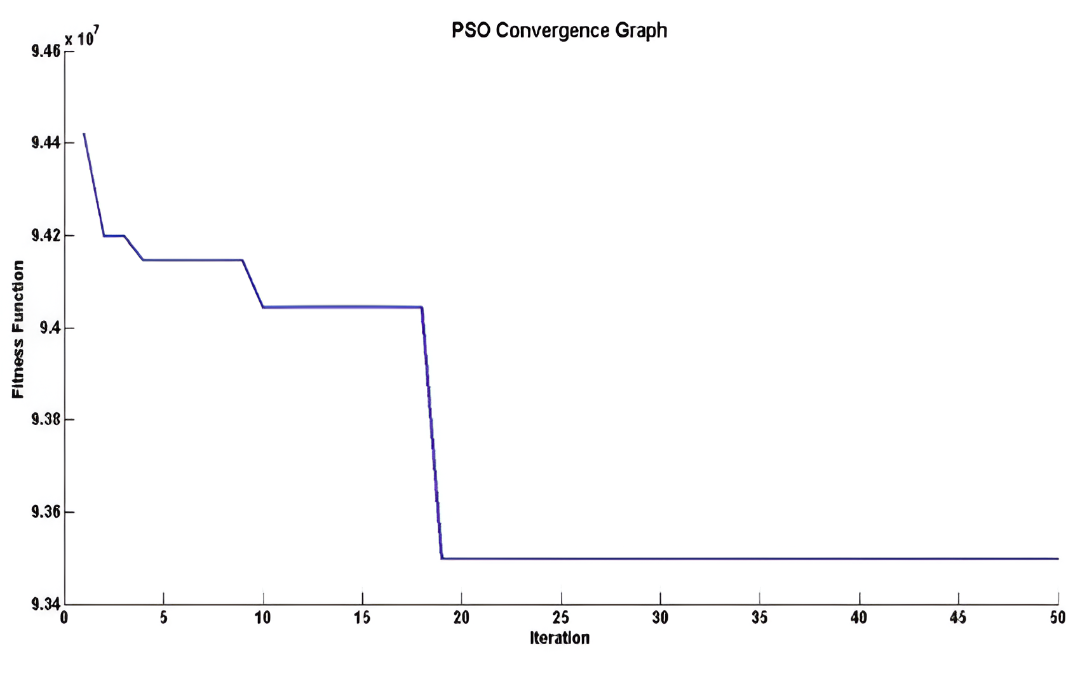
\includegraphics[width=\textwidth]{twse-rules-pso-optimization}
	\caption{Графики изменений максимального, среднего и лучшего по популяции значений оптимизируемой метрики.}
\end{figure}

Динамика максимального, среднего и лучшего по популяции значений оптимизируемой метрики в процессе PSO-оптимизации базы правил для подобранной выше комбинации гиперпараметров изображена на рисунке \cref{fig:twse-rules-pso-optimization}.

\begin{table} [htbp]% Пример записи таблицы с номером, но без отображаемого наименования
	\caption{Сравнение показателей качества прогнозирования временного ряда из набора данных TWSE (TAIEX).}%
	\label{tab:test1}%
	\begin{SingleSpace}
%			\begin{tabular}{| c{5cm} | *{2}{C{2.5cm}} | l *{3}{C{1.5cm}} |}
     \setlength\extrarowheight{2pt} %вот этим управляем расстоянием между рядами, \arraystretch даёт неудачный результат
\setlength{\tymin}{1.5cm}% минимальная ширина столбца
     \begin{tabulary}{\textwidth}{@{}>{\zz}C >{\zz}C >{\zz}C >{\zz}C >{\zz}C >{\zz}C@{}}% Вертикальные полосы не используются 	принципиально, как и лишние горизонтальные (допускается по ГОСТ 2.105 пункт 4.4.5) % @{} позволяет прижиматься к краям
			\toprule
			\multirow{2}{*}{Модель} & Время обучения, сек. & Время вывода, сек. & RMSE & MAPE & MAE \\
			\midrule
			MLP & -- & -- & 7.93     & 8.77     & 8.77     \\
			Decision Tree & -- & -- & 8.77     & 8.77     & 8.77     \\
			SVM & -- & -- & 8.77     & 8.77     & 8.77     \\
			ANFIS (Мамдани) & -- & -- & 8.77     & 8.77     & 8.77     \\
			ANFIS (Такаги-Сугено) & -- & -- & 8.77     & 8.77     & 8.77     \\
			\hline
			FTV-NSFLS+COG (упрощенная схема)        & 8.72     & 8.77     & 8.77     & 8.77     & 8.77     \\
			FTV-NSFLS+MeOM        & 8.72     & 8.77     & 8.77     & 8.77     & 8.77     \\
			\bottomrule
		\end{tabulary}%
	\end{SingleSpace}
\end{table}

\begin{figure}
	\centering
	%\includegraphics[scale=0.45]{twse-forecasting}
	\caption{Демонстрация предсказанных и фактических значений в наборе данных TWSE.}
	\label{fig:twse-forecasting}
\end{figure}

\cref{fig:twse-forecasting}

%Результат прогнозирования обученной нечеткой моделью изображен на рис. \cref{}.

\todo{На оборудовании ????? данная реализация имеет следующую производительность}

Конфигурация вычислительной системы: центральный процессор --- AMD Ryzen 9 5900HX (8 ядер, 16 потоков, базовая частота 3.3 ГГц, кэш L3 16 МБ); оперативная память --- 32 ГБ DDR4-3200 (двухканальный режим); графический процессор --- NVIDIA GeForce RTX 3080 Laptop GPU с 16 ГБ видеопамяти (CUDA 12.1, compute capability --- 8.6).


\section{Задача прогнозирования активности клиента по банковскому продукту}

Разработанная модель нечеткого логического вывода также была применена для прогнозирования оборотов юридических лиц по эквайрингу. Эквайринг --- 'это банковская услуга, позволяющая юридическим лицам принимать безналичные платежи от своих клиентов с помощью банковских карт и других платежных систем, таких как мобильные платежи (например, Mir Pay, Google Pay, Apple Pay) или QR-коды. Банк-эквайер предоставляет терминал, обрабатывает транзакции и переводит средства на счет юридического лица. Существует несколько основных видов эквайринга, каждый из которых предназначен для разных форматов бизнеса: торговый эквайринг --- самый распространенный вид, при котором в торговой точке устанавливается POS-терминал для приема карт (подходит для офлайн-магазинов, кафе и других предприятий, где оплата происходит при личном контакте с клиентом); интернет-эквайринг --- позволяет принимать платежи на сайтах, в мобильных приложениях и мессенджерах, для чего на сайт или в приложение интегрируется специальная платежная форма; мобильный эквайринг --- используются мобильные mPOS-терминалы, которые являются удобным решением для курьерских служб, такси, выездной торговли; оплата по QR-коду --- клиент сканирует QR-код с помощью своего мобильного устройства и подтверждает оплату в банковском приложении. Банк-эквайер взимает комиссию с каждой транзакции. Размер комиссии зависит от оборота юрлица, условий банка и типа используемой платёжной системы.

Прогнозирование объема транзакций по банковским продуктам позволяет подбирать более оптимальные условия обслуживания для клиента и принимать более точные решения по нему в различных ситуация. Прогнозные данные могут использоваться для различных целей:
\begin{enumerate}
	\item \textbf{Оценка кредитоспособности.} Прогноз оборота дает более точное и своевременное представление о финансовом состоянии компании, чем годовая отчетность. Если банк видит, что оборот клиента стабильно падает, это может быть ранним и главным сигналом о грядущих проблемах с погашением кредитов и возникновению просрочек.
	\item \textbf{Повышение прибыльности и оптимизация ценообразования.} Для клиентов с прогнозируемым высоким и стабильным оборотом банк может предложить более низкую комиссию по эквайрингу, чтобы удержать их и выиграть в конкурентной борьбе. И наоборот, для клиентов с нестабильным или падающим прогнозируемым оборотом можно сохранить стандартный или повышенный тариф. Анализ позволяет выявить компании с высоким потенциалом роста. Такие клиенты — главные кандидаты на углубление сотрудничества.
	\item \textbf{Своевременные предложения.} Если банк прогнозирует резкий рост оборота у клиента (например, сезонный всплеск у магазина подарков перед Новым годом), ему можно проактивно предложить краткосрочный кредит на пополнение оборотных средств.
	\item \textbf{Продажа дополнительных продуктов.} Растущему бизнесу могут потребоваться зарплатные проекты, корпоративные карты, новые расчетные счета или инвестиционные услуги. Прогноз позволяет сделать релевантное предложение в нужный момент.
	\item \textbf{Предотвращение оттока.} Если прогноз показывает стагнацию или падение оборота, менеджер может связаться с клиентом, чтобы выяснить причины и предложить решения (например, кредитные каникулы или реструктуризацию долга), тем самым повышая лояльность.
\end{enumerate}

Кроме того, банк может использовать агрегированные данные по всем корпоративным клиентам для анализа общей картины состояния рынка. Банк может видеть, какие отрасли экономики растут, а какие находятся в упадке, основываясь на совокупном обороте своих клиентов в этих секторах. Эта информация может использоваться для корректировки кредитной политики и маркетинговой стратегии.

Прогнозирование активности клиента по банковскому продукту (квайрингх.

 на \note[]{3} месяца вперед

Модель прогнозирования временных рядов строит прогноз с использованием значений только целевой переменной --- объема оборота юридических лиц по эквайрингу (авторегрессия). Набор данных составлен из помесячных значений временных рядов за период с 01-01-2021 по 31-12-2023 для 2500 уникальных клиентов. Из набора данных были удалены временные ряды, состоящие только из нулевых значений, то есть клиенты без активности по продукту. В результате осталось 1731 временных рядов.

В.

Для оценки качества прогнозирования была выбрана целевая метрика MAE --- данная метрика легко интерпретируема для данной задачи.

Размер лагового окна \todo{3, 5, 7, 11}.

\begin{table}[htbp]
	\centering
	\begin{threeparttable}% выравнивание подписи по границам таблицы
		\caption{Значения метрики MAE данной и альтернативных моделей.}%
		\label{tab:makecell}%
		\begin{tabular}{| c | c | c |}
			\toprule
			\multirow{2}{*}{Модель} & \multicolumn{2}{|c|}{Mean Absolute Error (MAE)} \\
			\cmidrule{2-3} & Среднее за \todo{3} мес. & Сумма за \todo{3} мес. \\
			\midrule
			Модель 1 & 1.0 & 2.0 \\
			Модель 2 & 1.0 & 2.0 \\
			Модель 3 & 1.0 & 2.0 \\
			FTV-NSFLS+MeOM & 1.0 & 2.0 \\
			\bottomrule
		\end{tabular}%
	\end{threeparttable}
\end{table}

\section{Описание набора данных}

\section{Решение задачи с использованием разработанной нечеткой модели}


\section{Выводы}